
\section{Análisis y especificación de requisitos}

Debido a la naturaleza autónoma de las estaciones meteorológicas, y a que el hecho que las mismas se encuentran sometidas a [something something] se busca crear un sistema centralizado de recolección de información que tenga gran tolerancia a las diversas condiciones adversas que se enfrentan las estaciones meteorológicas, a la vez que es lo suficientemente confiable para hacer un impacto positivo en la recolección de la información de las mismas.

\subsection{Conexión a estaciones remotas}

La conexión a las estaciones remotas se creó como un sistema modular de conexiones. Teniendo el objetivo de la extensibilidad como objetivo prioritario para el sistema de interacción con las interfaces.

Cada sistema de conexión supone sus propios retos, si bien hay diversos métodos de conexión que podrían ser útiles para la conexión a las estaciones meteorológicas, se decidió enfocarse en la conexión vía SSH a las estaciones meteorológicas que poseen una RaspberryPI como *datalogger* y como medio de interfaz que se encuentran conectadas por medio de puerto serial a las mismas. Y de las estaciones meteorológicas Campbell, que poseen diversos protocolos de comunicación pero se decidió por utilizar el protocolo HTTP.

Para la conexión a las estaciones RaspberryPi se considera lo siguiente:

\begin{itemize}
   \item Actualmente cuentan con una VPN configurada para facilitar el acceso a SSH por medio de una dirección IP en el mismo segmento de red que el segmento al que se pretende el servidor final tenga.
   \item Ocasionalmente, las estaciones meteorológicas perderán acceso a la VPN, ya sea por fallas técnicas del servidor, del ISP, pérdidas de energía eléctrica o demás.
   \item Que una estación se encuentre fuera de línea de la VPN temporalmente no implica que esta no pueda operar, o incluso que no pueda contactar al servidor, tal como se observa en la \ref{fig:conexion_redundancia}
\end{itemize}

\begin{figure}[!ht]
	\centering
	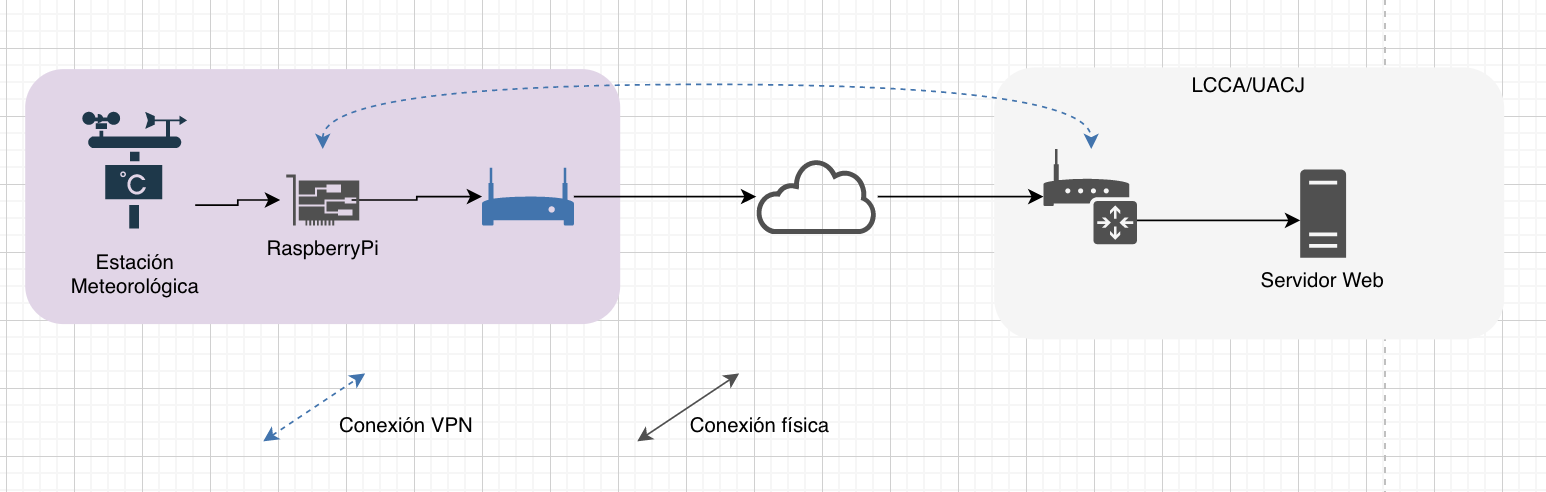
\includegraphics[width=.75\linewidth]{images/diagrams/conexion.png}
	\caption{Diagrama de la redundancia de las conexiones}
	\label{fig:conexion_redundancia}
\end{figure}

Por esta razón se optó por tener un servicio de monitoreo bidireccional. Se pretende que cambiando el ejecutor de servicios, se pueda obtener la información de la estación meteorológica sin necesidad de realizar diferentes implementaciones para cada caso. En este caso, se pretende que un script funcione en el mismo

\subsubsection{Consideraciones de seguridad}

Debido a que generalmente no se crea una red virtual privada separada para el manejo exclusivo de estaciones meteorológicas (ya que estas suelen instalarse sobre infraestructura existente) es importante tener consideraciones de seguridad respecto a el acceso a las estaciones, debido a que pueden ser un punto de acceso a una, otherwise, isolada y segura red.


\textbf{De la conexión del servidor a las estaciones meteorológicas}

Para realizar la conexión a las estaciones meteorológicas se requiere de acceso a la raspberrypi que funciona como puente entre ambas. Para realizar cambios, crear un servicio, y establecer la información del sistema con una mínima interacción se requiere de un usuario de alta prioridad a la máquina. En el caso del sistema operativo basado en linux que utilizan las estaciones, es el usuario con la mayor cantidad de procesos \emph{root}.

Al considerarse comprometido el ambiente de la apliación, se consideraría comprometido el sistema completo. Ya que en este ambiente se encontrarán las contraseñas de acceso a la base de datos y la llave privada que se utiliza para hacer autenticación, si bien existen servicios como Aws-KMS (Key Management Service), el implementar un sistema tan robusto para la administración de secretos sale de los objetivos de este proyecto.

Por lo tanto, se decidió crear un servicio que tome un usuario y password con acceso "root" de forma temporal (o al menos uno que tenga permisos de \emph{sudoer}) y utilizarlo para almacenar la llave pública local del servidor para realizar operaciones sin tener un usuario/password almacenado en la base de datos que pudiera ser comprometido. De esta forma, se mitiga el impacto de una posible intrusión a la base de datos, para no comprometer las credenciales de acceso a las estaciones.

\textbf{De las estaciones meteorológicas al servidor}

Debido a que las estaciones meteorológicas suelen ser instaladas en puntos con poco o mínimo control de seguridad física, se busca mitigar el acceso de las estaciones meteorológicas a la base de datos en la que se centralizarán los datos. Por lo tanto, se decidió utilizar un protocolo de API para insertar los eventos.


\subsection{Selección de herramientas}

Para el desarrollo de el proyecto, se decidió por realizar la aplicación de servidor con el lenguaje de programación Python. Esto debido a que otros proyectos de los que depende el funcionamiento de los sistemas de el LCCA, tales como el monitoreo climatológico y meteorológico con Weewx, y el proyecto para obtener la información de las estaciones meteorológicas en diferentes estándares fueron realizados con este lenguaje. Además, el lenguaje cuenta con una librería estándar extensa así como una librería de terceras partes madura que permite el desarrollo de forma sencilla utilizando estas librerías existentes, contando con la certeza de que están listas para un proyecto de producción.

%! TODO: Agregar referencias a las tesis de RapsberryPI y la de Alicia en el parrafito anterior.

El \textit{ORM} utilizado para el desarrollo de la aplicación, fué \textit{MasoniteORM}, un ORM para python que tiene como objetivos principales la simpleza y extendibilidad de proyectos. Si bien, \textit{MasoniteORM} es parte de \textit{Masonite}, un framework para el desarrollo de aplicaciones web, este es bastante extenso y complejo, y si bien es fácilmente extensible no es simple para usarse. Por lo tanto, se decidió utilizar el framework de desarrollo de aplicaciones web \textit{FastApi}, creado por Sebastián Ramírez (tiangolo), ya que ofrece una forma fácil de crear un \textit{API} web, el cuál será utilizado posteriormente para el desarrollo de una interfaz fácilmente accesible para los usuarios.

La interfaz gráfica para proveer acceso a la información a los usuarios se decidió hacer en una aplicación web. Esto debido a que las interfaces web ofrecen una amplia y madura plataforma desarrollo que se puede acceder desde diferentes tipos de dispositivos, así como una gran variedad de \textit{frameworks}, metodologías, y paradigmas, lo que ofrece una gran flexibilidad al momento de realizar un desarrollo a la medida. También está el hecho de que debido a la naturaleza del proyecto, un sistema que centraliza toda la información que es accesible por medio de un API, no parecía posible que un proyecto de una aplicación de escritorio o una aplicación web ofreciera una ventaja que no ofreciera la interfaz web.

VueJS

Por el motivo de hacer el proyecto lo más estándar, fácilmente acccesible y mantenible, se decidió realizar la programación y documentación del proyecto en inglés, pero manteniendo las interfaces en las que el usuario interactúa con el mismo en español. Además, se eligió el configurar \textit{pylint} con el estándar \textit{pep8} para el formato automático de el código del proyecto en el estándar. De la misma forma, se configuró \textit{ESLint} en el proyecto de VueJS para el fronted, extendiendo los estándares \textit{vue:essential} y \textit{eslint:recommended}, para realizar el formato automático en los archivos.
